\documentclass{article}

\usepackage[spanish]{babel}
\usepackage[numbers,sort&compress]{natbib}
\usepackage[T1]{fontenc}
\usepackage[ansinew]{inputenc}
\usepackage{graphicx}
\usepackage{url}
\usepackage{subcaption}
\usepackage{caption}
\usepackage{float}

\begin{document}
\title{\textbf{M\'etodo Monte Carlo}}
\author{Anahi Elizabeth Llano Guerrero}

\maketitle

\section{Objetivo}\label{obj}

El objetivo \cite{elisa} consiste en determinar el tama\~no de muestra requerido por cada lugar decimal de precisi\'on del estimado obtenido para el integral, comparando con Wolfram Alpha para por lo menos desde uno hasta siete decimales.

\section{Metodolog\'{i}a}\label{met}

Para determinar el tama\~no de muestra requerido para aumentar la precisi\'on del c\'alculo de la integral se us\'o R en su versi\'on 4.0.3.


La rutina se disen\'o variando el tama\~no de la muestra (10, 100, 1000, 10000, 100000) y realizando 100 repeticiones para cada uno de ellos.  Posteriormente se calcul\'o el error, que ser\'ia la diferencia entre el valor real y el obtenido por Monte-Carlo, grafic\'andolo en un diagrama de caja-bigote de tal manera que podamos observar la precisi\'on entre el n\'umero de decimales correctos y la aproximaci\'on obtenida por Monte-Carlo. El codigo utilizado se encuentra en el repositorio \cite{ana}.

\section{Resultados y Discusi\'{o}n}\label{res}

En la figura podemos observar el \'area debajo de las lineas se trata de la precisi\'on en cantidad de d\'igitos, por lo cual se observa que al aumentar los d\'igitos en la muestra podemos obtener m\'as precisi\'on de d\'igitos, por ejemplo cuando la muestra tiene un tama\~no de 100 y 1000, nuestra precisi\'on seria de dos d\'igitos, as\'i sucesivamente cuando la muestra es de 10,000 y 100,000 la precisi\'on seria en 3 d\'igitos, para 4 d\'igitos seria de 1,000,000, entonces mientras mayor sea el n\'umero de muestra mayor precisi\'on tendremos en los d\'igitos de la integral compar\'andola con la integral obtenida por Wolfram Alpha.


\begin{figure}[H]
       \centering
       \begin{subfigure}[b]{0.85\linewidth}
           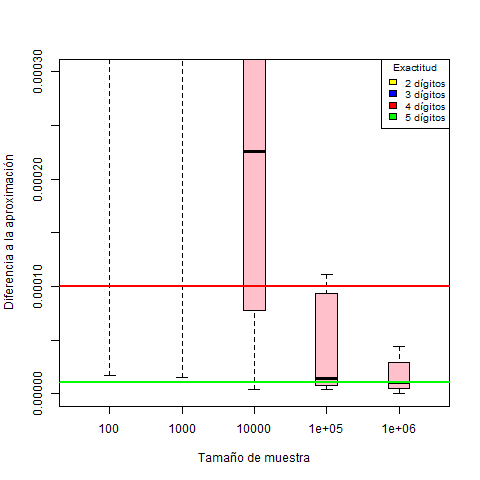
\includegraphics[width=\linewidth]{Grafica1.png}
           \caption{Tama\~no normal}
           \label{f1.a}
        \end{subfigure}
        \begin{subfigure}[b]{0.85\linewidth}
            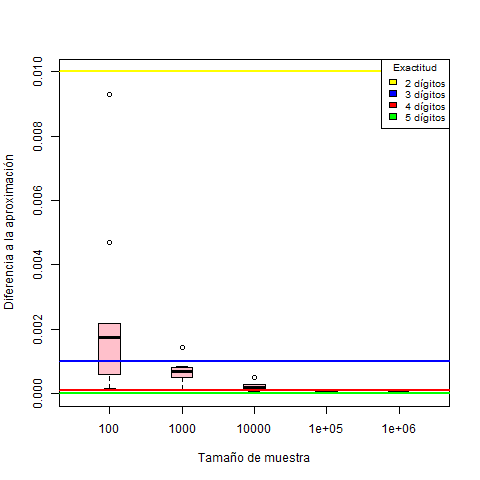
\includegraphics[width=\linewidth]{Grafica1.1.png}
            \caption{Amplida}
            \label{f1.b}
        \end{subfigure}
\caption{Diferencias entre el valor real y la aproximaci\'on de Monte Carlo}
        \label{f1}
\end{figure}

Se muestra la figura a y la figura b para poder observar de mejor manera la exactitud en los datos, en donde ambas figuras nos representan lo mismo, \'unicamente se vari\'o el tama\~no de la imagen para que fuera m\'as f\'acil visualizar cada una de las l\'ineas marcadas.
Se puede observar en la figura \ref{f1}, que mientras mayor sea en tama\~no de la muestra mayor ser\'a la aproximaci\'on al valor real, y esta exactitud se puede observar por el \'area abajo de la l\'inea aquellos que caen en la exactitud de 1 a 5 d\'igitos se encuentran en el \'area debajo de las l\'ineas de colores en donde cada color representa la exactitud de 1 hasta 5 d\'igitos, por lo tanto si quisi\'eramos ver esa exactitud entre el valor de Wolfran alpha y el valor calculado ser\'ia necesario tomar m\'as datos para la muestra, en este caso no se realiz\'o debido al tiempo de trabajo de la computadora en la que se trabaj\'o, ya que no tiene tanta capacidad para realizar trabajos tan grandes.


\section{Conclusi\'{o}n}\label{con}

El aumento en el tama\~no de la muestra tiene un efecto directo en la precisi\'on, cuando se intenta calcular una integral mediante el m\'etodo Monte Carlo.  Debido a que las muestras son tomadas de forma pseudoaleatoria al aumentar el tama\~no de muestra y las repeticiones aumenta la precisi\'on de la aproximaci\'on obtenida.

\section{Reto 1}\label{ret}

Para el primer reto consiste en implementar la estimaci\'on del valor de $\pi$ con el m\'etodo de Kurt, paralelizando con el tama\~no de la muestra para encontrar la relaci\'on matem\'atica entre estas y la precisi\'on obtenida en base a la cantidad de decimales correctos.
La t\'ecnica Kurt \citep{kurt} toma en cuenta el \'area del cuadrado y el \'area del circulo por lo que al efectuar la combinaci\'on y obtener un coeficiente se obtiene $\pi/4$  pudi\'endose asi obtener el valor de $\pi$ al multiplicarlo por 4 .
Se realiz\'o un procedimiento similar a la tarea base para calcular las aproximaciones entre el valor de $\pi$ y los valores generados, as\'i mismo en el diagrama de caja-bigote se tienen las cantidades decimales acertadas para la estimaci\'on de $\pi$.

\begin{figure}[H]
\begin{center}
\includegraphics[width=13cm]{exactpi.png}
\end{center}
\caption{ Comparaci\'on del tama\~no de muestra dependiendo del valor esperado y la cantidad de decimales acertadas en la
estimaci\'on de $\pi$. }
\label{f2}
\end{figure}

En la figura \ref{f2} se observan los resultados obtenidos donde es posible visualizar aquellos datos que caen dentro del valor aproximado a $\pi$  en donde se muestra de igual manera que mientras mayor sean los valores generados mayor ser\'a la aproximaci\'on a este. Dados los resultados anteriores podr\'iamos concluir que el m\'etodo Monte-Carlo se basa en que a mayor cantidad en el tama\~no de la muestra o bien puntos generados, se va incrementado el acercamiento con el valor real, aunque tambi\'en podr\'ian depender el n\'umero de decimales con el tama\~o de la muestra ya que el comportamiento en este caso fue similar a el presentado en la tarea base, y en este caso se obtuvieron valores donde la precisi\'on se present\'o en hasta 6 decimales pero el tama\~no de la muestra fue un tama\~no promedio para obtener la exactitud en estos, por lo cual en este caso se podr\'ia rechazar la idea de que mientras mayor sea el tama\~no de la muestra mayor ser\'a la precisi\'on en el c\'alculo.

  \bibliography{P5}
  \bibliographystyle{plainnat}
\end{document}